\chapter{Anhang}
	\begin{lstlisting}[style=python, caption={Zur Auswertung der konduktometrischen Titration verwendeter Python-Code.}]
		import matplotlib.pyplot as plt
		import numpy as np
		import pandas as pd
		from scipy.optimize import curve_fit
		import os

		sample_files = os.listdir("messdaten/csv_titration/")
		print(sample_files)

		spl_lst = []
		for i,file in enumerate(sample_files):
			with open(("messdaten/csv_titration/" + file), newline='', encoding='utf-8') as path:
				frame = pd.read_csv(path, delimiter=';')
				frame.columns = [col.strip() for col in frame] # stupid whitespaces t(-_-t)
				spl_lst.append(frame)
				del frame

		absorb = spl_lst[0]
		known = spl_lst[1]
		absorb_vol = np.array(absorb["Vol. Maßlösung / [mL]"])
		absorb_leit = np.array(absorb["Leitfähigkeit / [mS/cm]"])
		known_vol = np.array(known["Vol. Maßlösung / [mL]"])
		known_leit = np.array(known["Leitfähigkeit / [uS/cm]"])

		def func(x, m, b):
			return x*m+b

		def findx(m, b, n, c):
			return (b - c)/(n - m)

		cm = 1/2.54 # inch to cm, metric like brrr

		plt.style.use("default")
		plt.style.use("seaborn-paper")

		fig1, ax1 = plt.subplots(figsize=(20*cm, 20*(9/16)*cm))

		ax1.scatter(absorb["Vol. Maßlösung / [mL]"], absorb["Leitfähigkeit / [mS/cm]"],
		marker="x", linewidth=.6, label="Datenpunkte")
		popt, pcov = curve_fit(func, np.array(absorb_vol[0:np.argmin(absorb_leit)-1]), np.array(absorb_leit[0:np.argmin(absorb_leit)-1]))
		m, b = popt
		ax1.plot(np.array(absorb_vol[0:np.argmin(absorb_leit)+8]),
		func(np.array(absorb_vol[0:np.argmin(absorb_leit)+8]), *popt),
		color="#800000", linestyle="--", label="Lin. Fit")
		popt, pcov = curve_fit(func, np.array(absorb_vol[np.argmin(absorb_leit)-1:]), np.array(absorb_leit[np.argmin(absorb_leit)-1:]))
		n, c = popt
		ax1.plot(np.array(absorb_vol[np.argmin(absorb_leit)-2:]),
		func(np.array(absorb_vol[np.argmin(absorb_leit)-2:]) ,*popt),
		color="#800000", linestyle="--")
		ax1.axvline(findx(m, b, n, c), lw=0.5, color="#800000", label="Verbr. Vol. $\\approx$ 9.461 mL")

		ax1.set_title("Verlauf der Leitfähigkeit - Absorberlösung aus V11", fontsize=12)
		ax1.set_xticks(np.arange(0,23,2))
		ax1.set_xlabel("Vol. Maßlösung / $mL$", fontsize=8)
		ax1.set_ylabel("Leitfähigkeit / $\\frac{mS}{cm}$", fontsize=8)
		ax1.legend()
		ax1.grid(axis='both', alpha=.3)
		#========================================================
		fig2, ax2 = plt.subplots(figsize=(20*cm, 20*(9/16)*cm))

		ax2.scatter(known["Vol. Maßlösung / [mL]"], known["Leitfähigkeit / [uS/cm]"],
		marker="x", linewidth=.6, label="Datenpunkte")
		popt, pcov = curve_fit(func, np.array(known_vol[0:np.argmin(known_leit)-1]), np.array(known_leit[0:np.argmin(known_leit)-1]))
		m, b = popt
		ax2.plot(np.array(known_vol[0:np.argmin(known_leit)+4]),
		func(np.array(known_vol[0:np.argmin(known_leit)+4]), *popt),
		color="#800000", linestyle="--", label="Lin. Fit")
		popt, pcov = curve_fit(func, np.array(known_vol[np.argmin(known_leit):]), np.array(known_leit[np.argmin(known_leit):]))
		n, c = popt
		ax2.plot(np.array(known_vol[np.argmin(known_leit)-1:]),
		func(np.array(known_vol[np.argmin(known_leit)-1:]) ,*popt),
		color="#800000", linestyle="--")
		ax2.axvline(findx(m, b, n, c), lw=0.5, color="#800000", label="Verbr. Vol. $\\approx$ 24.788 mL")
		# print(findx(m, b, n, c))

		ax2.set_title("Verlauf der Leitfähigkeit - Chloridlösung", fontsize=12)
		ax2.set_xticks(np.arange(0,46,5))
		ax2.set_xlabel("Vol. Maßlösung / $mL$", fontsize=8)
		ax2.set_ylabel("Leitfähigkeit / $\\frac{\\mu S}{cm}$", fontsize=8)
		ax2.legend()
		ax2.grid(axis='both', alpha=.3)

		plt.tight_layout()
		plt.show()
	\end{lstlisting}
	\clearpage
	\begin{lstlisting}[style=python, caption={Zur Auswertung der kalorimetrischen Messung verwendeter Python-Code.}]
		import matplotlib.pyplot as plt
		import numpy as np
		import pandas as pd
		from scipy.optimize import curve_fit
		import os

		sample_files = os.listdir("messdaten/csv_kalo/")
		print(sample_files)

		spl_lst = []
		for i,file in enumerate(sample_files):
			with open(("messdaten/csv_kalo/" + file), newline='', encoding='utf-8') as path:
				frame = pd.read_csv(path, delimiter=';')
				frame.columns = [col.strip() for col in frame] # whitespaces, again! double t(-_-t)
				spl_lst.append(frame)
				del frame

		kalib = spl_lst[0]
		benzo = spl_lst[1]
		kalib_zeit = np.array(kalib["Zeit"] * 60)
		kalib_temp = np.array(kalib["Temp"] + 273.15)
		benzo_zeit = np.array(benzo["Zeit"] * 60)
		benzo_temp = np.array(benzo["Temp"] + 273.15)
		
		cm = 1/2.54 # inch to cm, metric like brrr

		plt.style.use("seaborn-paper")

		fig1, ax1 = plt.subplots(figsize=(20*cm, 20*(9/16)*cm))

		ax1.plot(kalib_zeit, kalib_temp,
		label=("Kalibrierung, $\Delta T = {:.4f}K$".format(np.max(kalib_temp)-np.min(kalib_temp))))
		ax1.plot(benzo_zeit, benzo_temp,
		label=("Probe, $\Delta T = {:.4f}K$".format(np.max(benzo_temp)-np.min(benzo_temp))), color="#800000")

		ax1.set_title("Temperaturänderung der kalorimetrischen Bestimmung", fontsize=12)
		ax1.set_xlabel("Zeit / [s]", fontsize=8)
		ax1.set_ylabel("Temperatur / [K]", fontsize=8)
		ax1.axhline(np.min(kalib_temp), linestyle="--", lw=.5)
		ax1.axhline(np.max(kalib_temp), linestyle="--", lw=.5)
		ax1.axhline(np.min(benzo_temp), linestyle="--", lw=.5, color="#800000")
		ax1.axhline(np.max(benzo_temp), linestyle="--", lw=.5, color="#800000")
		ax1.legend(loc=4)
		ax1.grid(axis='both', alpha=.3)

		plt.tight_layout()
		plt.show()
	\end{lstlisting}
	\clearpage
	\begin{figure}[h]
		\centering
		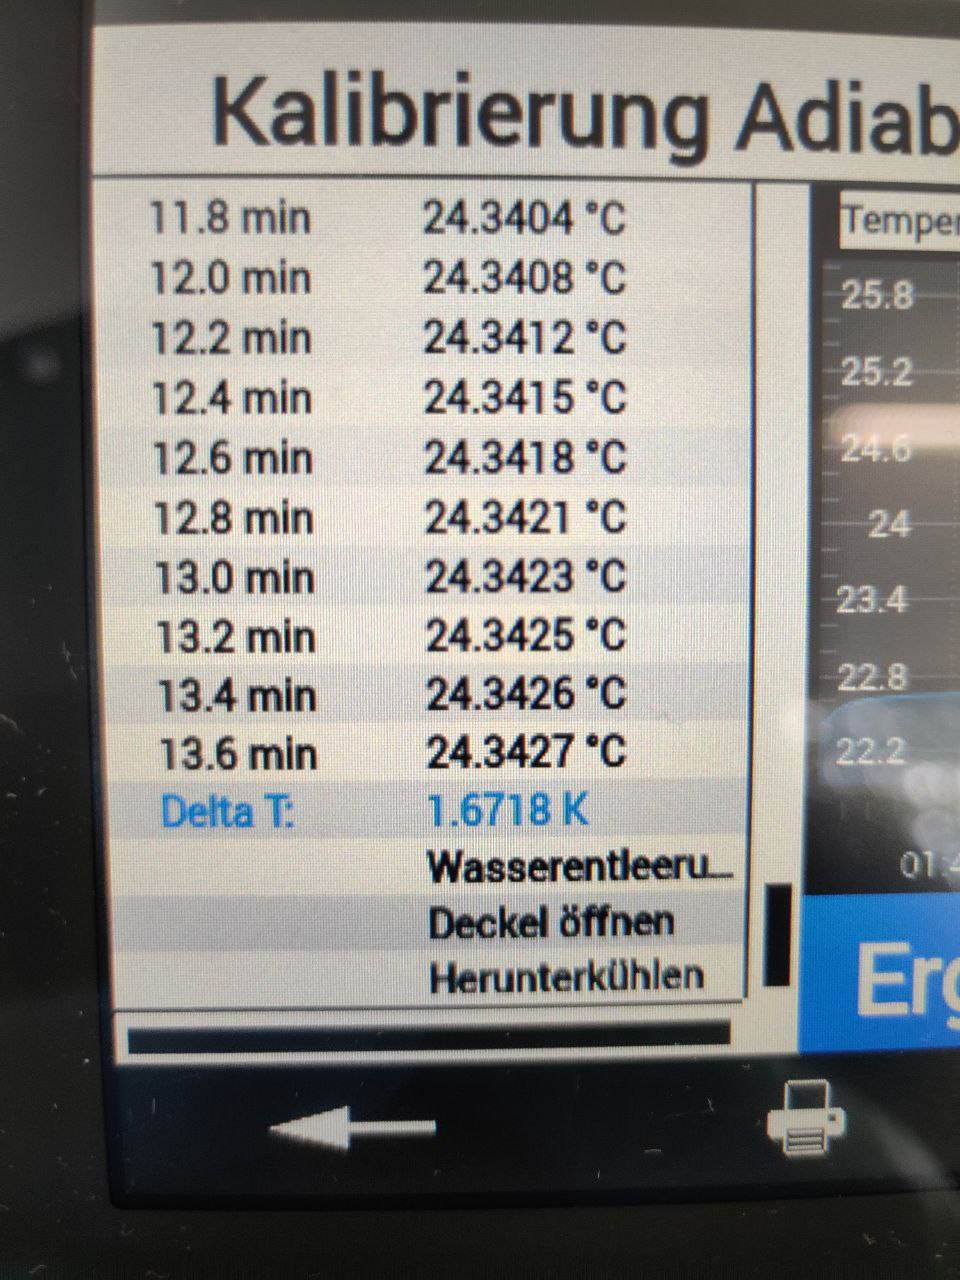
\includegraphics[width=.8\textwidth]{assets/photos/kaloriemeter_kalib5.jpg}
		\caption[Gemessene Temperaturdifferenz des Kalibriervorgangs]{Gemessene Temperaturdifferenz des Kalibriervorgangs.}
		\label{fig:gemessene temperaturdifferenz des kalibriervorgangs}
	\end{figure}
	\begin{figure}[h]
		\centering
		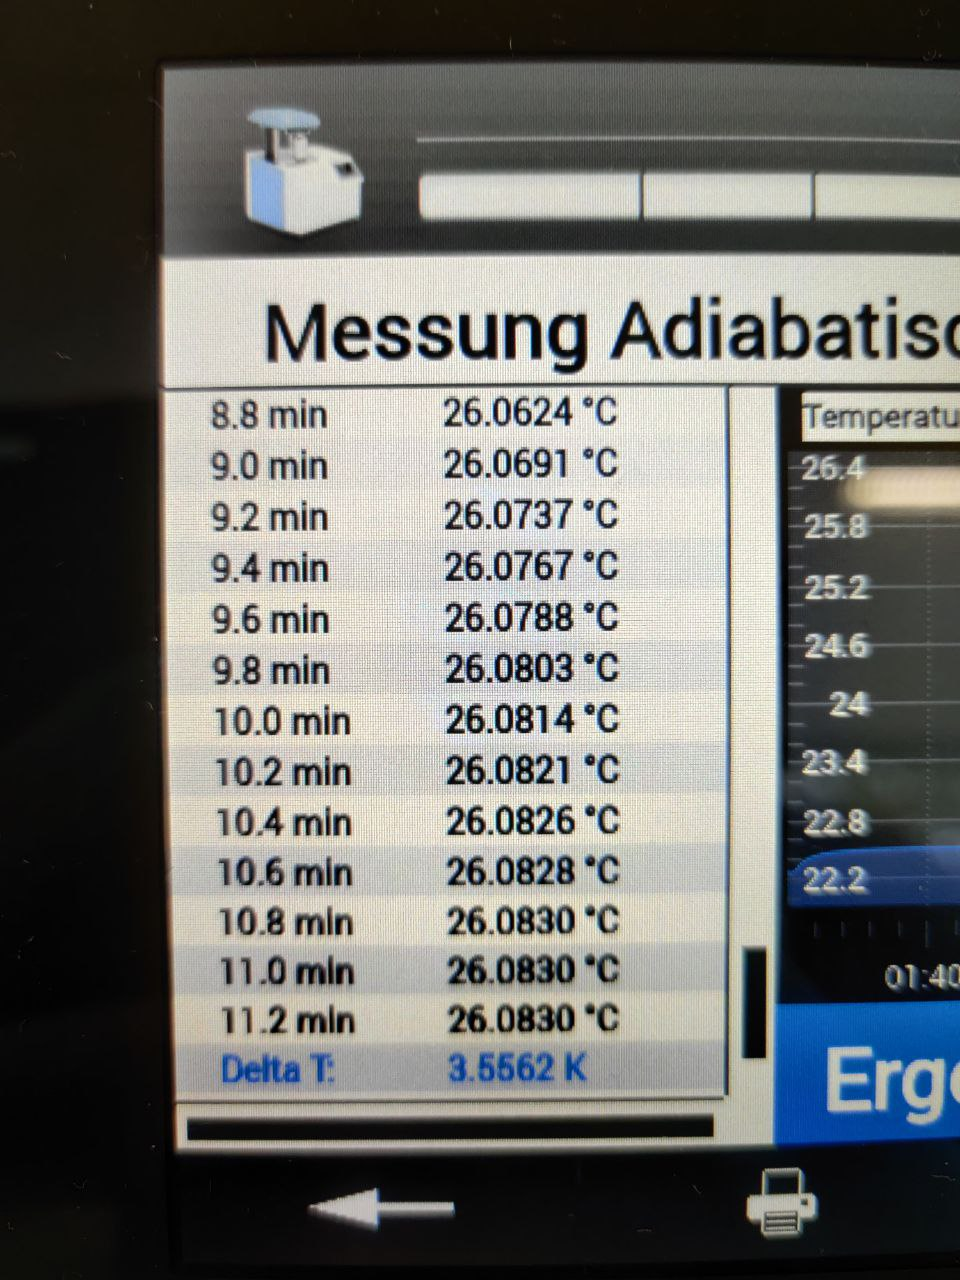
\includegraphics[width=.8\textwidth]{assets/photos/kaloriemeter_messung3.jpg}
		\caption[Gemessene Temperaturdifferenz der Probenmessung]{Gemessene Temperaturdifferenz der Probenmessung.}
		\label{fig:gemessene temperaturdifferenz der probenmessung}
	\end{figure}